% !TeX program = xelatex
\documentclass[12pt, a4paper]{article}
\usepackage{amsmath}
\usepackage{xeCJK}
\usepackage{amsmath}
\usepackage{amssymb}
\usepackage{tikz}
\usepackage{xcolor}
\usepackage{parskip}
\usepackage{enumitem}


\setmainfont{Latin Modern Roman}
\setCJKmainfont{Noto Serif CJK TC}

\title{Vector analysis}

\begin{document}
\subsection*{Divergence Teorem}
$$
\int_{V} \nabla \cdot \vec{A} \text{d}v = \oint_{s} \vec{A} \text{d} \vec{s}
$$

\textbf{Definition}: The volume integral of the divergence of a vector filed equals the total outward flux of the viector through the surface that bounds the volume.

$$
\nabla \cdot \vec{A} \triangleq \lim_{\Delta v \to 0} {\frac{\oint_{s} \vec{A} \text{d} \vec{s}}{\Delta v}}
$$
\\
Directly
$$
\Rightarrow (\nabla \cdot \vec{A})_{j} \Delta V_{j} = \oint_{S_j} \vec{A} \text{d} \vec{s}
$$
\\ 
A very small differential volume element $\Delta V_j$ bounded by a surface $S_j$
\\






\tikzset{every picture/.style={line width=0.75pt}} %set default line width to 0.75pt        

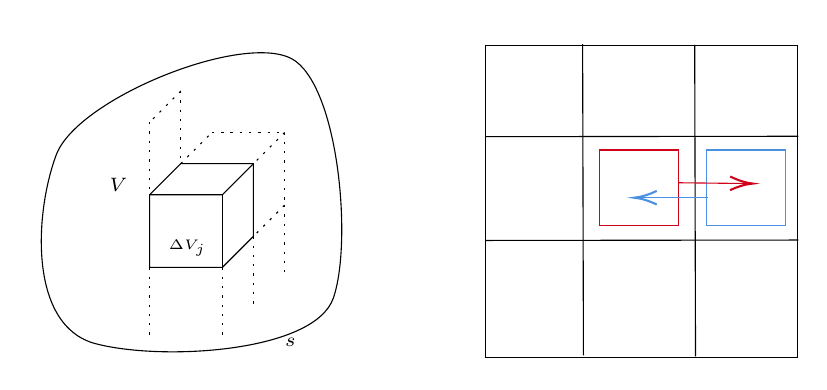
\begin{tikzpicture}[x=0.75pt,y=0.75pt,yscale=-1,xscale=1]
%uncomment if require: \path (0,300); %set diagram left start at 0, and has height of 300

%Shape: Cube [id:dp7404291900565326] 
\draw   (228,142) -- (243,127) -- (278,127) -- (278,162) -- (263,177) -- (228,177) -- cycle ; \draw   (278,127) -- (263,142) -- (228,142) ; \draw   (263,142) -- (263,177) ;
%Straight Lines [id:da9158926856096958] 
\draw  [dash pattern={on 0.84pt off 2.51pt}]  (243,127) -- (258,112) ;
%Straight Lines [id:da9560584623286865] 
\draw  [dash pattern={on 0.84pt off 2.51pt}]  (258,112) -- (293,112) ;
%Straight Lines [id:da47387905157318244] 
\draw  [dash pattern={on 0.84pt off 2.51pt}]  (293,112) -- (278,127) ;
%Straight Lines [id:da8241605675800876] 
\draw  [dash pattern={on 0.84pt off 2.51pt}]  (293,112) -- (293,147) ;
%Straight Lines [id:da11079411968427466] 
\draw  [dash pattern={on 0.84pt off 2.51pt}]  (293,147) -- (278,162) ;
%Straight Lines [id:da2360709880742038] 
\draw  [dash pattern={on 0.84pt off 2.51pt}]  (293,147) -- (293,182) ;
%Straight Lines [id:da524366771962634] 
\draw  [dash pattern={on 0.84pt off 2.51pt}]  (278,162) -- (278,178) -- (278,197) ;
%Straight Lines [id:da3064489344701309] 
\draw  [dash pattern={on 0.84pt off 2.51pt}]  (263,177) -- (263,212) ;
%Straight Lines [id:da11276393412081243] 
\draw  [dash pattern={on 0.84pt off 2.51pt}]  (228,177) -- (228,212) ;
%Straight Lines [id:da300889570362631] 
\draw  [dash pattern={on 0.84pt off 2.51pt}]  (243,92) -- (243,127) ;
%Straight Lines [id:da718875838380094] 
\draw  [dash pattern={on 0.84pt off 2.51pt}]  (228,107) -- (228,142) ;
%Straight Lines [id:da5301915554623988] 
\draw  [dash pattern={on 0.84pt off 2.51pt}]  (243,92) -- (228,107) ;
%Shape: Polygon Curved [id:ds8813539032718901] 
\draw   (183,122.75) .. controls (193.5,94.75) and (277.5,61.75) .. (298.5,77.75) .. controls (319.5,93.75) and (325.5,165.75) .. (316.5,191.75) .. controls (307.5,217.75) and (234.5,222.25) .. (202,213.75) .. controls (169.5,205.25) and (172.5,150.75) .. (183,122.75) -- cycle ;
%Shape: Rectangle [id:dp641843266142239] 
\draw   (390,70.2) -- (540,70.2) -- (540,220.2) -- (390,220.2) -- cycle ;
%Straight Lines [id:da5199911184615083] 
\draw    (436.6,69.4) -- (437,219.4) ;
%Straight Lines [id:da03620576215856386] 
\draw    (490.6,69.8) -- (491,219.8) ;
%Straight Lines [id:da20381395101040423] 
\draw    (390,114) -- (540.6,113.8) ;
%Straight Lines [id:da11280171069834277] 
\draw    (390,164) -- (540.6,163.8) ;
%Shape: Rectangle [id:dp09580199404468714] 
\draw  [color={rgb, 255:red, 208; green, 2; blue, 27 }  ,draw opacity=1 ] (444.8,120.4) -- (482.6,120.4) -- (482.6,157) -- (444.8,157) -- cycle ;
%Shape: Rectangle [id:dp4813629624838279] 
\draw  [color={rgb, 255:red, 74; green, 144; blue, 226 }  ,draw opacity=1 ] (496.4,120.4) -- (534.2,120.4) -- (534.2,157) -- (496.4,157) -- cycle ;
%Straight Lines [id:da31091752492015057] 
\draw [color={rgb, 255:red, 208; green, 2; blue, 27 }  ,draw opacity=1 ]   (482.8,136.2) -- (516.6,136.58) ;
\draw [shift={(518.6,136.6)}, rotate = 180.64] [color={rgb, 255:red, 208; green, 2; blue, 27 }  ,draw opacity=1 ][line width=0.75]    (10.93,-3.29) .. controls (6.95,-1.4) and (3.31,-0.3) .. (0,0) .. controls (3.31,0.3) and (6.95,1.4) .. (10.93,3.29)   ;
%Straight Lines [id:da040152325850278836] 
\draw [color={rgb, 255:red, 74; green, 144; blue, 226 }  ,draw opacity=1 ]   (496.8,143.4) -- (463.4,143.4) ;
\draw [shift={(461.4,143.4)}, rotate = 360] [color={rgb, 255:red, 74; green, 144; blue, 226 }  ,draw opacity=1 ][line width=0.75]    (10.93,-3.29) .. controls (6.95,-1.4) and (3.31,-0.3) .. (0,0) .. controls (3.31,0.3) and (6.95,1.4) .. (10.93,3.29)   ;

% Text Node
\draw (236,162.4) node [anchor=north west][inner sep=0.75pt]  [font=\tiny]  {$\Delta V_{j}$};
% Text Node
\draw (292,209.9) node [anchor=north west][inner sep=0.75pt]  [font=\scriptsize]  {$s$};
% Text Node
\draw (207.5,132.9) node [anchor=north west][inner sep=0.75pt]  [font=\scriptsize]  {$V$};
\end{tikzpicture}
\\ 




\begin{align*}
	\color{blue} \lim_{\Delta V_j \to 0}(\sum_{j=1}^{N} \color{black} (\nabla \cdot \vec{A}_j) \Delta V_j \color{blue}) \color{black} &= \color{blue} \lim_{\Delta V_j \to 0} \sum_{j=1}^{N} \color{black} \oint_{S_j} \vec{A} \text{d} \vec{s} \\
	\int_{V} (\nabla \cdot \vec{A}) \text{d} v &= \oint_{s} \vec{A} \text{d} \vec{s}
\end{align*}

\newpage
\section*{Curl of a vector field}
$\nabla \cdot \vec{A}$: a measure of the strength of the flow source vortex source: a circulatior of a vector around it. \\

Circulation of $\vec{A}$ around countour $C \triangleq \oint_C \vec{A} \text{d} \vec{l}$ \\

\textbf{Physical meaning:}

\begin{enumerate}[label=\textcircled{\arabic*}]
	\item $\vec{A} \cdot$ force ($\vec{F}$) $\to \oint_C \vec{A} \text{d} \cdot \vec{l}$ :\quad  work
	
	\item $\vec{A}$; electrical field intensity $\to \oint_C \vec{A} \cdot \text{d} \vec{l}$ :\quad electromotive force
\end{enumerate}

$\nabla \times \vec{A}$ (curl $\vec{A}$): a measure of strength of a vector source \\ 

\textbf{magnitude:} The maximum net circulation of $\vec{A}$ per unit area as the area tends to zero. \\
\textbf{direction:} The normal direction of the area when the area is oriented to make the net circulation maxium.

\subsection*{Stokes's Theorem}

\begin{center}


\tikzset{every picture/.style={line width=0.75pt}} %set default line width to 0.75pt        

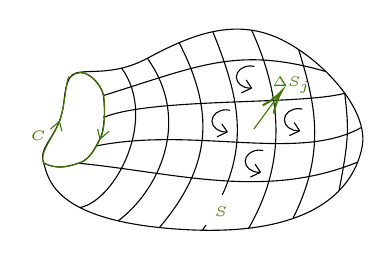
\begin{tikzpicture}[x=0.75pt,y=0.75pt,yscale=-1,xscale=1]
%uncomment if require: \path (0,300); %set diagram left start at 0, and has height of 300

%Shape: Polygon Curved [id:ds9570049595220438] 
\draw   (280.5,106.25) .. controls (283.15,101.31) and (292.48,104.61) .. (305.6,101.5) .. controls (309.43,100.58) and (313.59,99.12) .. (318,96.75) .. controls (318.85,96.29) and (319.7,95.84) .. (320.55,95.39) .. controls (324.78,93.16) and (329.03,91.07) .. (333.29,89.25) .. controls (338.67,86.96) and (344.07,85.1) .. (349.53,83.95) .. controls (355.7,82.65) and (361.94,82.27) .. (368.24,83.21) .. controls (371.48,83.69) and (374.73,84.52) .. (378,85.75) .. controls (382.15,87.31) and (386.53,89.64) .. (390.86,92.51) .. controls (395.4,95.53) and (399.89,99.15) .. (403.97,103.13) .. controls (407.36,106.43) and (410.47,109.97) .. (413.11,113.62) .. controls (417.04,119.03) and (419.93,124.66) .. (421.17,130.04) .. controls (421.91,133.23) and (422.06,136.33) .. (421.5,139.25) .. controls (421.04,141.68) and (420.34,144.2) .. (419.33,146.75) .. controls (417.49,151.44) and (414.62,156.21) .. (410.32,160.6) .. controls (405.18,165.84) and (398.01,170.54) .. (388.09,173.97) .. controls (382.06,176.05) and (375.02,177.65) .. (366.81,178.62) .. controls (360.2,179.39) and (352.82,179.75) .. (344.59,179.6) .. controls (341.67,179.55) and (338.64,179.43) .. (335.5,179.25) .. controls (331.34,179.01) and (327.45,178.69) .. (323.8,178.3) .. controls (316.13,177.49) and (309.55,176.38) .. (303.91,175.07) .. controls (296.15,173.26) and (290.16,171.06) .. (285.51,168.68) .. controls (270.31,160.89) and (269.47,151.21) .. (268,147.25) .. controls (265.6,140.78) and (272,136.25) .. (275.5,127.25) .. controls (279,118.25) and (277.08,112.64) .. (280.5,106.25) -- cycle ;
%Curve Lines [id:da7038238403142679] 
\draw    (280.5,106.25) .. controls (287,98.7) and (296,109.3) .. (296.8,114.7) .. controls (297.26,117.79) and (297.45,122.65) .. (297.09,127.11) .. controls (296.81,130.43) and (296.23,133.53) .. (295.2,135.5) .. controls (294.61,136.63) and (294.01,137.81) .. (293.36,138.99) .. controls (291.36,142.6) and (288.88,146.09) .. (284.8,147.3) .. controls (284.44,147.41) and (284.09,147.51) .. (283.74,147.62) .. controls (278.81,149.09) and (274.54,150.29) .. (268,147.25) ;
%Curve Lines [id:da808813885485639] 
\draw    (305.6,101.5) .. controls (323.4,126.1) and (302.4,165.5) .. (285.51,168.68) ;
%Curve Lines [id:da835490412177286] 
\draw    (318,96.75) .. controls (339.8,127.3) and (323,160.9) .. (303.91,175.07) ;
%Curve Lines [id:da9618135436614953] 
\draw    (333.29,89.25) .. controls (349.8,121.3) and (350,147.5) .. (323.8,178.3) ;
%Curve Lines [id:da5661778835850406] 
\draw    (349.53,83.95) .. controls (364.8,121.5) and (367.4,144.5) .. (344.59,179.6) ;
%Curve Lines [id:da26048077431163286] 
\draw    (368.24,83.21) .. controls (382.8,115.3) and (385.4,146.3) .. (366.81,178.62) ;
%Curve Lines [id:da8623873632827426] 
\draw    (390.86,92.51) .. controls (398.4,117.1) and (404.8,140.7) .. (388.09,173.97) ;
%Curve Lines [id:da9804592457238139] 
\draw    (413.11,113.62) .. controls (414.8,129.7) and (415.6,133.7) .. (410.32,160.6) ;
%Curve Lines [id:da9303324302436777] 
\draw    (296.8,114.7) .. controls (342.6,100.5) and (361.17,90.75) .. (403.97,103.13) ;
%Curve Lines [id:da2177407237482134] 
\draw    (296.83,125.25) .. controls (320.41,115.56) and (391.17,119.42) .. (413.11,113.62) ;
%Curve Lines [id:da40561561694164605] 
\draw    (293.36,138.99) .. controls (340.83,129.42) and (391.17,147.08) .. (421.17,130.04) ;
%Curve Lines [id:da07223211772381188] 
\draw    (284.8,147.3) .. controls (331.5,151.92) and (374.67,165.08) .. (419.33,146.75) ;
%Curve Lines [id:da06900651334327179] 
\draw [color={rgb, 255:red, 65; green, 117; blue, 5 }  ,draw opacity=1 ]   (280.64,106.28) .. controls (287.14,98.73) and (296.14,109.33) .. (296.94,114.73) .. controls (297.4,117.82) and (297.6,122.68) .. (297.23,127.13) .. controls (296.96,130.46) and (296.37,133.56) .. (295.34,135.53) .. controls (294.76,136.66) and (294.16,137.84) .. (293.51,139.02) .. controls (291.5,142.63) and (289.02,146.12) .. (284.94,147.33) .. controls (284.59,147.43) and (284.24,147.54) .. (283.89,147.64) .. controls (278.95,149.12) and (274.68,150.31) .. (268.14,147.28) ;
%Curve Lines [id:da820963534781842] 
\draw [color={rgb, 255:red, 65; green, 117; blue, 5 }  ,draw opacity=1 ]   (280.64,106.28) .. controls (279.11,102.61) and (278.51,119.94) .. (275.64,127.28) .. controls (272.78,134.61) and (265.44,142.94) .. (268.14,147.28) ;
%Straight Lines [id:da27998789730506113] 
\draw [color={rgb, 255:red, 65; green, 117; blue, 5 }  ,draw opacity=1 ]   (271.3,130.88) -- (275.5,127.25) ;
%Straight Lines [id:da7371646762729195] 
\draw [color={rgb, 255:red, 65; green, 117; blue, 5 }  ,draw opacity=1 ]   (275.64,127.28) -- (276.84,131.94) ;
%Straight Lines [id:da5786556978235863] 
\draw [color={rgb, 255:red, 65; green, 117; blue, 5 }  ,draw opacity=1 ]   (295.34,135.53) -- (299.54,131.89) ;
%Straight Lines [id:da3376088344414613] 
\draw [color={rgb, 255:red, 65; green, 117; blue, 5 }  ,draw opacity=1 ]   (294,130.83) -- (295.2,135.5) ;
%Straight Lines [id:da3897337244745851] 
\draw [color={rgb, 255:red, 65; green, 117; blue, 5 }  ,draw opacity=1 ]   (369.29,130.86) -- (381.53,114.18) ;
\draw [shift={(382.71,112.57)}, rotate = 126.29] [color={rgb, 255:red, 65; green, 117; blue, 5 }  ,draw opacity=1 ][line width=0.75]    (10.93,-3.29) .. controls (6.95,-1.4) and (3.31,-0.3) .. (0,0) .. controls (3.31,0.3) and (6.95,1.4) .. (10.93,3.29)   ;
%Shape: Arc [id:dp10789944624851777] 
\draw  [draw opacity=0] (368.2,111.12) .. controls (368.02,111.14) and (367.83,111.14) .. (367.64,111.14) .. controls (363.9,111.14) and (360.86,108.74) .. (360.86,105.79) .. controls (360.86,102.83) and (363.9,100.43) .. (367.64,100.43) .. controls (368.29,100.43) and (368.92,100.5) .. (369.52,100.64) -- (367.64,105.79) -- cycle ; \draw   (368.2,111.12) .. controls (368.02,111.14) and (367.83,111.14) .. (367.64,111.14) .. controls (363.9,111.14) and (360.86,108.74) .. (360.86,105.79) .. controls (360.86,102.83) and (363.9,100.43) .. (367.64,100.43) .. controls (368.29,100.43) and (368.92,100.5) .. (369.52,100.64) ;  
%Straight Lines [id:da23629965748646042] 
\draw    (368.2,111.12) -- (363.29,113.43) ;
%Straight Lines [id:da42134393246415136] 
\draw    (368.2,111.12) -- (365.57,107.14) ;
%Shape: Arc [id:dp3040002611916668] 
\draw  [draw opacity=0] (356.49,132.27) .. controls (356.3,132.28) and (356.12,132.29) .. (355.93,132.29) .. controls (352.18,132.29) and (349.14,129.89) .. (349.14,126.93) .. controls (349.14,123.97) and (352.18,121.57) .. (355.93,121.57) .. controls (356.58,121.57) and (357.21,121.64) .. (357.8,121.78) -- (355.93,126.93) -- cycle ; \draw   (356.49,132.27) .. controls (356.3,132.28) and (356.12,132.29) .. (355.93,132.29) .. controls (352.18,132.29) and (349.14,129.89) .. (349.14,126.93) .. controls (349.14,123.97) and (352.18,121.57) .. (355.93,121.57) .. controls (356.58,121.57) and (357.21,121.64) .. (357.8,121.78) ;  
%Straight Lines [id:da6031003036106222] 
\draw    (356.49,132.27) -- (351.57,134.57) ;
%Straight Lines [id:da47716762346415276] 
\draw    (356.49,132.27) -- (353.86,128.29) ;
%Shape: Arc [id:dp9055322787067043] 
\draw  [draw opacity=0] (372.49,151.7) .. controls (372.3,151.71) and (372.12,151.71) .. (371.93,151.71) .. controls (368.18,151.71) and (365.14,149.32) .. (365.14,146.36) .. controls (365.14,143.4) and (368.18,141) .. (371.93,141) .. controls (372.58,141) and (373.21,141.07) .. (373.8,141.21) -- (371.93,146.36) -- cycle ; \draw   (372.49,151.7) .. controls (372.3,151.71) and (372.12,151.71) .. (371.93,151.71) .. controls (368.18,151.71) and (365.14,149.32) .. (365.14,146.36) .. controls (365.14,143.4) and (368.18,141) .. (371.93,141) .. controls (372.58,141) and (373.21,141.07) .. (373.8,141.21) ;  
%Straight Lines [id:da0744871945350295] 
\draw    (372.49,151.7) -- (367.57,154) ;
%Straight Lines [id:da06372935088999188] 
\draw    (372.49,151.7) -- (369.86,147.71) ;
%Shape: Arc [id:dp4569628769412635] 
\draw  [draw opacity=0] (391.35,131.7) .. controls (391.16,131.71) and (390.97,131.71) .. (390.79,131.71) .. controls (387.04,131.71) and (384,129.32) .. (384,126.36) .. controls (384,123.4) and (387.04,121) .. (390.79,121) .. controls (391.44,121) and (392.06,121.07) .. (392.66,121.21) -- (390.79,126.36) -- cycle ; \draw   (391.35,131.7) .. controls (391.16,131.71) and (390.97,131.71) .. (390.79,131.71) .. controls (387.04,131.71) and (384,129.32) .. (384,126.36) .. controls (384,123.4) and (387.04,121) .. (390.79,121) .. controls (391.44,121) and (392.06,121.07) .. (392.66,121.21) ;  
%Straight Lines [id:da6440322537618585] 
\draw    (391.35,131.7) -- (386.43,134) ;
%Straight Lines [id:da34063719289590955] 
\draw    (391.35,131.7) -- (388.71,127.71) ;

% Text Node
\draw (260.6,130.3) node [anchor=north west][inner sep=0.75pt]  [font=\tiny,color={rgb, 255:red, 65; green, 117; blue, 5 }  ,opacity=1 ]  {$C$};
% Text Node
\draw (377.14,104.4) node [anchor=north west][inner sep=0.75pt]  [font=\fontsize{0.35em}{0.42em}\selectfont,color={rgb, 255:red, 65; green, 117; blue, 5 }  ,opacity=1 ]  {$\Delta S_{j}$};
% Text Node
\draw  [color={rgb, 255:red, 255; green, 255; blue, 255 }  ,draw opacity=1 ][fill={rgb, 255:red, 255; green, 255; blue, 255 }  ,fill opacity=1 ]  (346.14,162.71) -- (364.14,162.71) -- (364.14,176.71) -- (346.14,176.71) -- cycle  ;
\draw (349.14,167.11) node [anchor=north west][inner sep=0.75pt]  [font=\tiny,color={rgb, 255:red, 65; green, 117; blue, 5 }  ,opacity=1 ]  {$S$};
\end{tikzpicture}
\end{center}
\begin{align*}
	&\because (\nabla \times \vec{A})_u = \hat{a_u} \cdot (\nabla \times \vec{A}) = \lim_{\Delta S_u \to 0} \frac{1}{\Delta S_u} (\oint_{Cu} \vec{A} \text{d} \vec{l})\\
	&\therefore (\nabla \times \vec{A})_j \cdot (\Delta S_j) = \oint_{C_j} \vec{A} \text{d} \vec{l}
\end{align*}
$\Delta S_j$: a very small differential area \\
$\oint_{C_j}$: bounded by a contour $C_j$

\begin{align*}
	\lim_{\Delta S_j \to 0} \sum_{j=1}^{N}(\nabla \times \vec{A})_j\cdot (\Delta S_j) &= \lim_{\Delta S_j \to 0} \sum_{j=1}^{N}(\oint_{C_j} \vec{A} \text{d} \vec{l}) \\
	\int_{S} (\nabla \times \vec{A}) \cdot \text{d} \vec{s} &= \oint _C \vec{A} \cdot \text{d} \vec{l}
\end{align*}


\newpage
\textbf{Exercise 2-14}
$$
\vec{F} = \hat{a_x}xy - \hat{a_y}2x
$$
Find out $\oint_{OABO} = \vec{F} \cdot \text{d} \vec{l}$.


\tikzset{every picture/.style={line width=0.75pt}} %set default line width to 0.75pt        

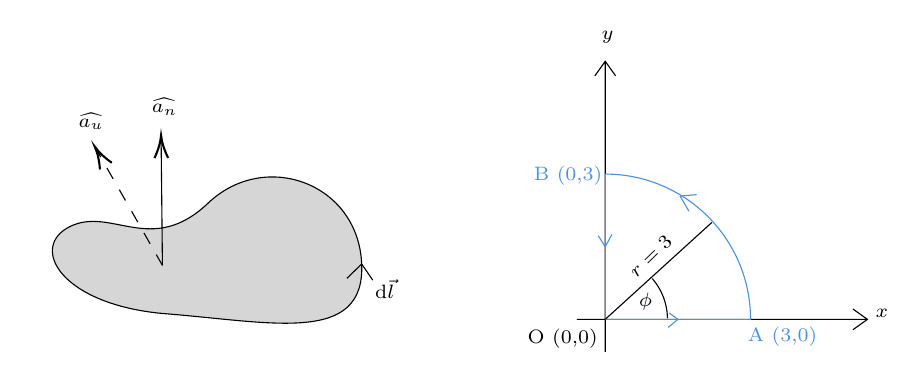
\begin{tikzpicture}[x=0.75pt,y=0.75pt,yscale=-1,xscale=1]
%uncomment if require: \path (0,300); %set diagram left start at 0, and has height of 300

%Shape: Polygon Curved [id:ds02407968906442648] 
\draw  [fill={rgb, 255:red, 0; green, 0; blue, 0 }  ,fill opacity=0.16 ] (89.67,108.33) .. controls (109.67,98.33) and (129,123) .. (156.33,97) .. controls (183.67,71) and (228.67,87.33) .. (230.33,126.33) .. controls (232,165.33) and (187,154.33) .. (136.33,150.33) .. controls (85.67,146.33) and (69.67,118.33) .. (89.67,108.33) -- cycle ;
%Straight Lines [id:da23150186547280338] 
\draw    (134.33,127) -- (133.69,66.33) ;
\draw [shift={(133.67,64.33)}, rotate = 89.39] [color={rgb, 255:red, 0; green, 0; blue, 0 }  ][line width=0.75]    (10.93,-3.29) .. controls (6.95,-1.4) and (3.31,-0.3) .. (0,0) .. controls (3.31,0.3) and (6.95,1.4) .. (10.93,3.29)   ;
%Straight Lines [id:da560950628707298] 
\draw  [dash pattern={on 4.5pt off 4.5pt}]  (134.33,127) -- (102.66,71.4) ;
\draw [shift={(101.67,69.67)}, rotate = 60.33] [color={rgb, 255:red, 0; green, 0; blue, 0 }  ][line width=0.75]    (10.93,-3.29) .. controls (6.95,-1.4) and (3.31,-0.3) .. (0,0) .. controls (3.31,0.3) and (6.95,1.4) .. (10.93,3.29)   ;
%Straight Lines [id:da8872557045790619] 
\draw    (223.22,133.22) -- (230.33,126.33) ;
%Straight Lines [id:da7034351428090797] 
\draw    (230.33,126.33) -- (235.67,134.11) ;
%Shape: Axis 2D [id:dp5560459976336004] 
\draw  (334,153) -- (474,153)(347.67,28.67) -- (347.67,168.67) (467,148) -- (474,153) -- (467,158) (342.67,35.67) -- (347.67,28.67) -- (352.67,35.67)  ;
%Shape: Arc [id:dp548460921370604] 
\draw  [draw opacity=0] (347.67,83) .. controls (347.67,83) and (347.67,83) .. (347.67,83) .. controls (386.33,83) and (417.67,114.34) .. (417.67,153) -- (347.67,153) -- cycle ; \draw  [color={rgb, 255:red, 74; green, 144; blue, 226 }  ,draw opacity=1 ] (347.67,83) .. controls (347.67,83) and (347.67,83) .. (347.67,83) .. controls (386.33,83) and (417.67,114.34) .. (417.67,153) ;  
%Straight Lines [id:da5563582787778145] 
\draw [color={rgb, 255:red, 74; green, 144; blue, 226 }  ,draw opacity=1 ]   (347.67,83) -- (347.67,153) ;
%Straight Lines [id:da663779790843842] 
\draw [color={rgb, 255:red, 74; green, 144; blue, 226 }  ,draw opacity=1 ]   (347.67,153) -- (417.67,153) ;
%Straight Lines [id:da32593798912107075] 
\draw [color={rgb, 255:red, 74; green, 144; blue, 226 }  ,draw opacity=1 ]   (383.75,93.63) -- (388,100.88) ;
%Straight Lines [id:da3581954407033726] 
\draw [color={rgb, 255:red, 74; green, 144; blue, 226 }  ,draw opacity=1 ]   (383.75,93.63) -- (391.75,92.88) ;
%Straight Lines [id:da8635416407668947] 
\draw [color={rgb, 255:red, 74; green, 144; blue, 226 }  ,draw opacity=1 ]   (344.25,112.63) -- (347.67,118) ;
%Straight Lines [id:da9827578661170833] 
\draw [color={rgb, 255:red, 74; green, 144; blue, 226 }  ,draw opacity=1 ]   (347.67,118) -- (350.92,112) ;
%Straight Lines [id:da37584167121294254] 
\draw [color={rgb, 255:red, 74; green, 144; blue, 226 }  ,draw opacity=1 ]   (378,156.88) -- (382.67,153) ;
%Straight Lines [id:da7626811673129976] 
\draw [color={rgb, 255:red, 74; green, 144; blue, 226 }  ,draw opacity=1 ]   (378.5,149.88) -- (382.67,153) ;
%Straight Lines [id:da9263467270455434] 
\draw    (347.67,153) -- (399,106.33) ;
%Shape: Arc [id:dp2641779136900759] 
\draw  [draw opacity=0] (370.31,133.32) .. controls (374.79,138.46) and (377.54,145.15) .. (377.66,152.48) -- (347.67,153) -- cycle ; \draw   (370.31,133.32) .. controls (374.79,138.46) and (377.54,145.15) .. (377.66,152.48) ;  

% Text Node
\draw (128,45.07) node [anchor=north west][inner sep=0.75pt]  [font=\scriptsize]  {$\widehat{a_{n}}$};
% Text Node
\draw (92.67,52.07) node [anchor=north west][inner sep=0.75pt]  [font=\scriptsize]  {$\widehat{a_{u}}$};
% Text Node
\draw (235.5,132.4) node [anchor=north west][inner sep=0.75pt]  [font=\scriptsize]  {$\text{d}\vec{l}$};
% Text Node
\draw (415.14,155.57) node [anchor=north west][inner sep=0.75pt]  [font=\scriptsize,color={rgb, 255:red, 74; green, 144; blue, 226 }  ,opacity=1 ] [align=left] {A (3,0)};
% Text Node
\draw (312,78.05) node [anchor=north west][inner sep=0.75pt]  [font=\scriptsize,color={rgb, 255:red, 74; green, 144; blue, 226 }  ,opacity=1 ] [align=left] {B (0,3)};
% Text Node
\draw (309.05,156.43) node [anchor=north west][inner sep=0.75pt]  [font=\scriptsize,color={rgb, 255:red, 0; green, 0; blue, 0 }  ,opacity=1 ] [align=left] {O (0,0)};
% Text Node
\draw (476.67,146.73) node [anchor=north west][inner sep=0.75pt]  [font=\scriptsize]  {$x$};
% Text Node
\draw (344.67,12.73) node [anchor=north west][inner sep=0.75pt]  [font=\scriptsize]  {$y$};
% Text Node
\draw (356.65,128.78) node [anchor=north west][inner sep=0.75pt]  [font=\scriptsize,rotate=-316.01]  {$r=3$};
% Text Node
\draw (362.57,139.11) node [anchor=north west][inner sep=0.75pt]  [font=\scriptsize]  {$\phi $};
\end{tikzpicture}

\textbf{Sol.} \\
\begin{align*}
	\oint_{OABO} = \vec{F} \cdot \text{d} \vec{l} \\
	\Rightarrow \int_{O}^{A} + \int_{A}^{B} + \int_{B}^{O}
\end{align*}

For $BO$: 
\begin{align*}
	x = 0, \quad
	\vec{F} = 0, \quad
	\int_{B}^{O} \vec{F} \cdot \text{d} \vec{l} = 0
\end{align*}

For $OA$:
	\begin{align*}
	&y = 0, \quad
	\vec {F} = - \hat{a_y} 2x, \quad
	\text{d} \vec{l} = \hat{a_x} \text{d} x \\
	&\therefore \vec{F} \cdot \text{d} \vec{l} = 0, \quad
	\therefore \int_{O}^{A} \vec{F} \cdot \vec{l} = 0
\end{align*}

For $AB$
\begin{align*}
	\text{d} \vec{l} = \hat{a_x} \text{d}x &+ \hat{a_y} \text{d}y, \quad
	\vec{F} \cdot \text{d} \vec{l} = xy \text{d}x -2x \text{d}y, \quad
	\text{since } x^{2} + y^{2} = 9 \\
	\int_{A}^{B} \vec{F} \cdot \text{d} \vec{l}
	&= \int_{3}^{0} xy \text{d}x - \int_{0}^{3} 2x \text{d}y
	= \int_{3}^{0} x \sqrt{9-x^{2}} \text{d}x - 2\int_{0}^{3} \sqrt{9-y^2} \text{d}y \\
	&=\left. -\frac{1}{3}(9-x^2)^{\frac{3}{2}} \right|_3^0 - \left.[y \sqrt{9-y^2} + 9\sin^{-1}\frac{y}{3} \right]_0^3\\
	&= -9(1 + \frac{\pi}{2})
\end{align*}
\newpage

\section*{Two null identities}
\subsection*{Identity \romannumeral1}
$\nabla \times (\nabla V) \equiv 0$ the curl of the gradient of any scalar field is identically zero \\
\begin{align*}
	&\int_{s} (\nabla \times (\nabla V)) \cdot \text{d} \vec{s} = oint_{C} (\nabla V) \cdot \text{d} \vec{l} \\ 
	&\text{By Stokes's theorem, we have} \\
	&\int_{s} (\nabla \times \vec{A}) \text{d} \vec{s} = \oint_{C} \vec {A} \cdot \text{d} \vec{l} \\
	\because &(\nabla V) \cdot \text{d} \vec{l} = \text{d} = \text{d} v \\
	\therefore &\oint_C \text{d} V = 0
\end{align*}



\end{document}
